%%=============================================================================
%% Methodologie
%%=============================================================================

\chapter{\IfLanguageName{dutch}{Methodologie}{Methodology}}%
\label{ch:methodologie}

Het onderzoek begint met een grondige literatuurstudie, beschreven in Hoofdstuk 2 van de methodologie. Deze studie geeft een overzicht van de beschikbare technologieën en methoden om teksten te vereenvoudigen voor leerlingen met dyslexie in de derde graad van het middelbaar onderwijs. Het doel van de literatuurstudie is om de lezer de benodigde kennis te bieden om de analyse-resultaten te begrijpen en biedt een duidelijke uiteenzetting van de verschillende aspecten van het onderzoek. Hoofdstuk 4 presenteert een lijst van functionaliteiten die beschikbaar zijn bij verschillende tools om teksten te vereenvoudigen voor leerlingen met dyslexie. Er wordt gekeken naar de capaciteiten en functionaliteiten van de tools en op basis hiervan wordt een shortlist van benodigde functionaliteiten opgesteld om teksten te vereenvoudigen voor leerlingen in de derde graad van het middelbaar onderwijs met dyslexie. Hoofdstuk 5 beschrijft het stappenplan voor de ontwikkeling van een prototype voor tekstvereenvoudiging. Het prototype houdt rekening met de benodigde functionaliteiten en eigenschappen die uit de requirementsanalyse voortvloeiden. De tool wordt lokaal opgezet. Hoofdstuk 6 presenteert een vergelijkende studie waarin verschillende tools worden vergeleken. De tools worden gebruikt om een wetenschappelijk artikel te vereenvoudigen of samen te vatten. De laatste fase van het onderzoek beantwoordt welke tools het meest geschikt zijn om wetenschappelijke artikelen voor leerlingen met dyslexie in de derde graad van het middelbaar onderwijs te vereenvoudigen. De tools worden afgetoetst op basis van de metrieken en vereisten die in hoofdstuk 2 worden besproken, met als doel te bepalen aan welke criteria een vereenvoudigde tekst moet voldoen om leerlingen met dyslexie in de derde graad van het middelbaar onderwijs te ondersteunen.

\chapter{Requirementsanalyse}

In deze fase van het onderzoek worden tools getest. Functionele eigenschappen die in Hoofdstuk 2 als nuttig zijn beschouwd, worden opgenomen in de requirementsanalyse. Aspecten waar ontwikkelaars bewust van moeten zijn worden in de requirementsanalyse opgenomen. De requirementsanalyse is opgesplitst tussen applicaties die nu in het onderwijs worden gebruikt en online tools die leraren in het onderwijs kunnen gebruiken.

\section{Tekstanalyse}

Geen enkel softwarepakket of hulpmiddel biedt standaard een visuele weergave van waarom een taal- of AI-model een zin als moeilijk of belangrijk beschouwt, of waarom het model een kernwoord heeft gekozen. Dit komt overeen met de bevindingen van \textcite{Gooding2019}. Het GPT3-model en het verwante Bing-model doen dit echter wel wanneer het taalmodel hier expliciet om wordt gevraagd. SciSpace houdt hier geen rekening mee en verwerpt de vraag. Het stellen van vragen aan het taalmodel biedt weliswaar een alternatief, maar valt buiten het bereik en de capaciteiten van de gemiddelde gebruiker. Deze prompt kan worden aangeboden in de vorm van een intuïtieve knop. 

Simplish geeft nadien een vergelijkende weergave met de oorspronkelijke tekst en de vereenvoudigde tekst. Met gebruik van kleurcodes worden de verschillende transformaties aangeduid.

\begin{figure}[H]
	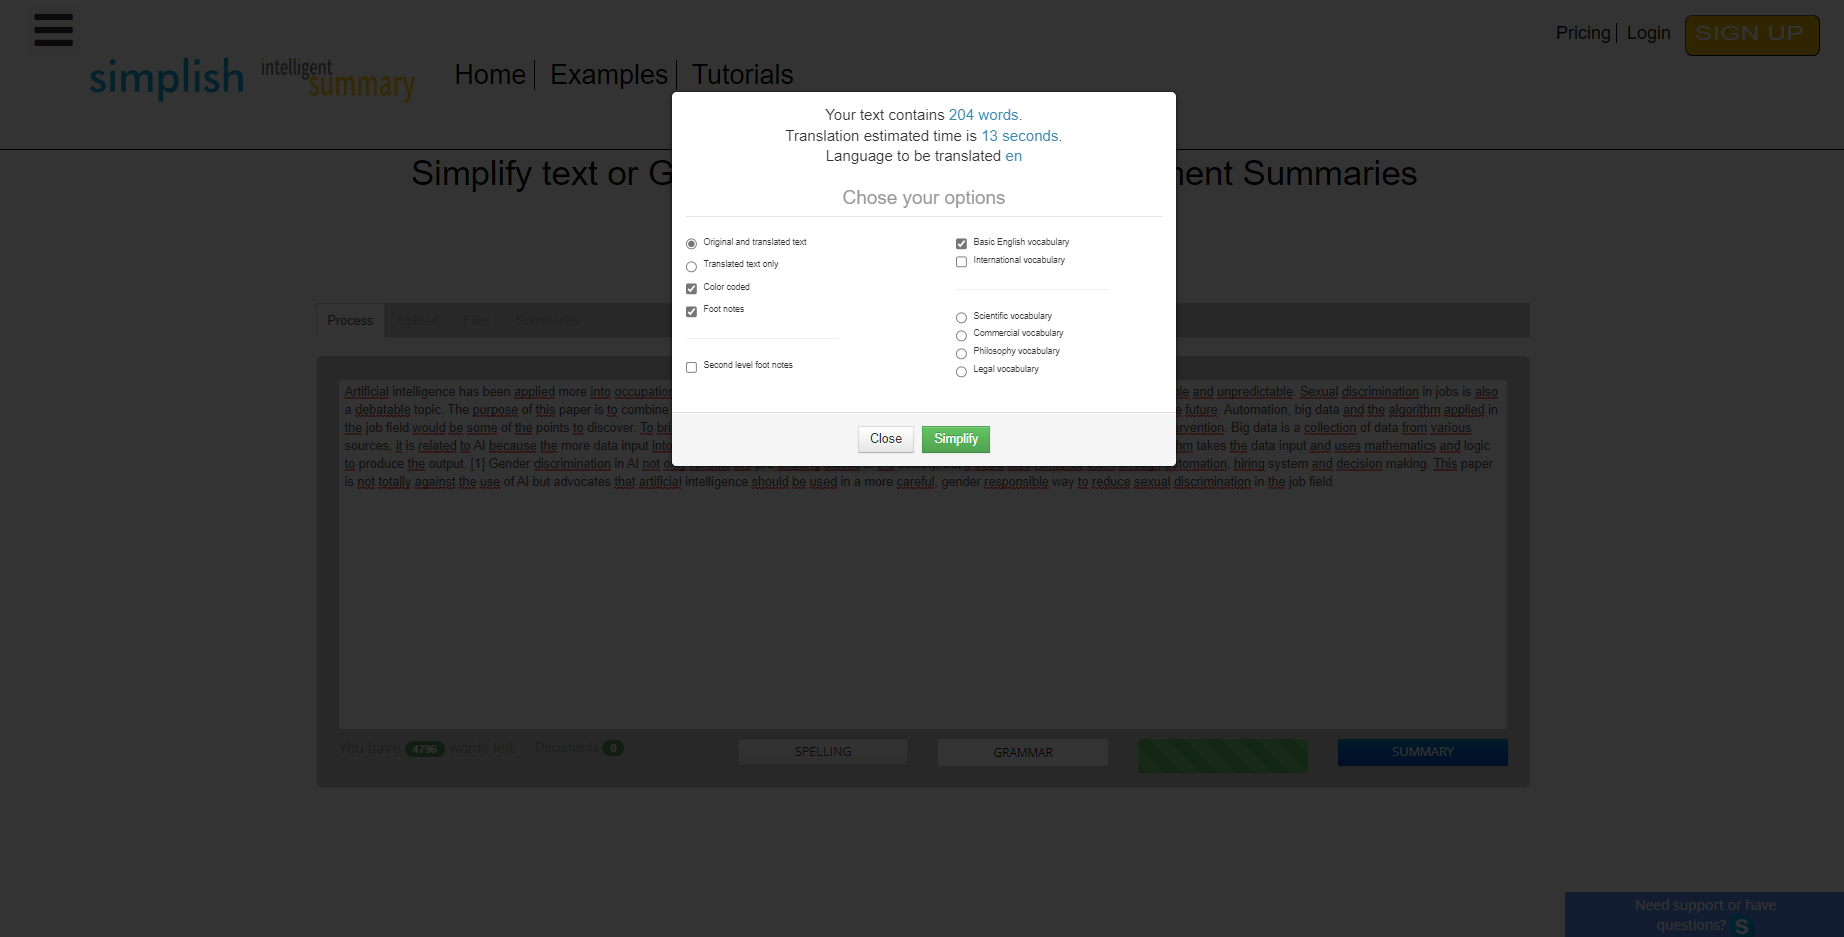
\includegraphics[width=\linewidth]{img/simplish-input.png}
\end{figure}

\begin{figure}[H]
	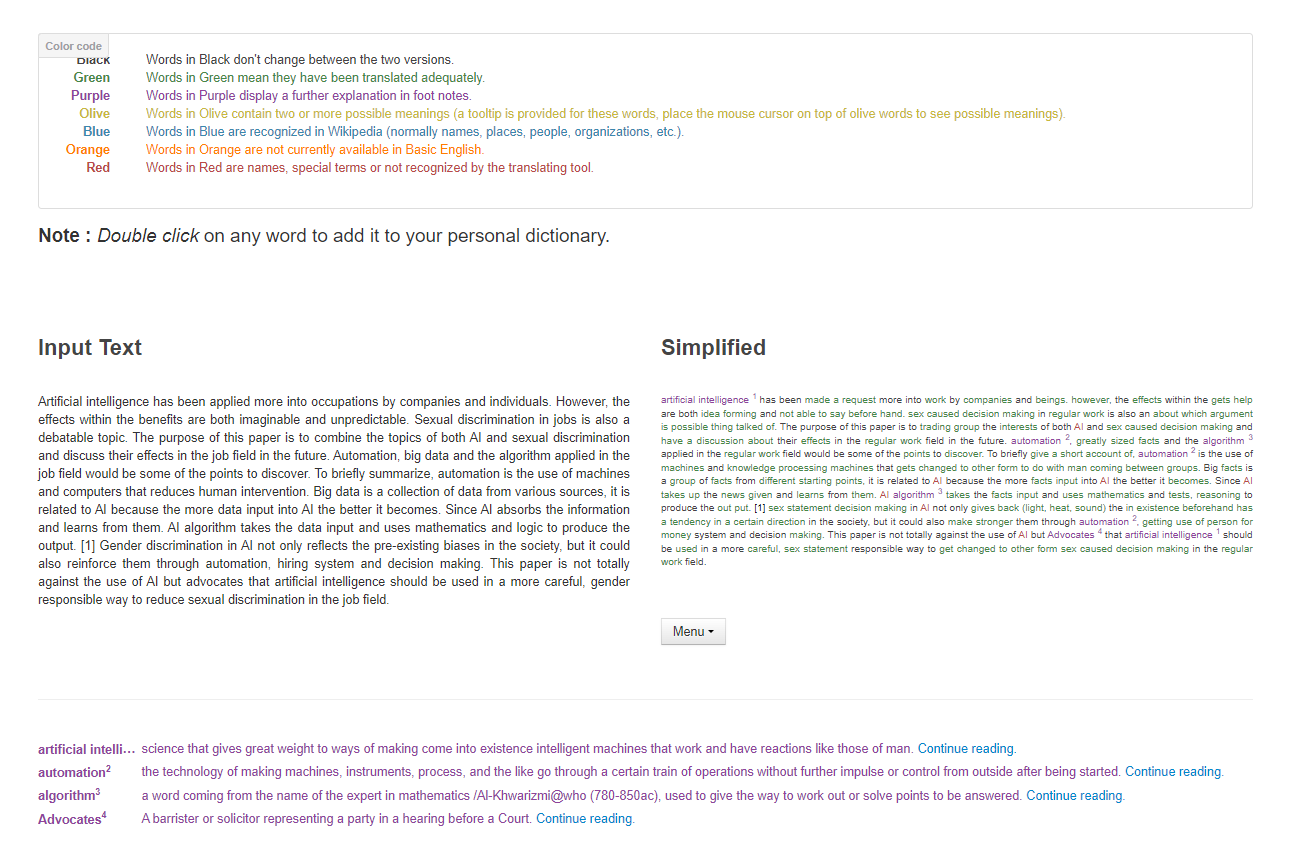
\includegraphics[width=\linewidth]{img/simplish-output.png}
\end{figure}

\section{Lexicale vereenvoudiging}

Huidige software in het onderwijs ingezet is in staat om woordenlijsten op te maken. Kurzweil biedt de functionaliteit om meer informatie te geven over een door de gebruiker gekozen woord, soortgelijk aan de werking van een woordenboek. Daarnaast biedt Kurzweil ook de mogelijkheid om als eindgebruiker de bron of woordenboek te kiezen waarvan de definitie moet worden opgehaald. Complexe woorden worden echter niet automatisch herkend door het systeem. Transformaties aan de woordenschat van een tekst komen in deze softwarepakketten niet aan bod.

\begin{table}[H]
	\centering
	\resizebox{0.8\textwidth}{!}{
	\begin{tabular}{|p{2cm}|l|l|l|l|l|l|}
		\hline
		Onderwerp & Mv & Sp & K3000 & AS & IW & TA \\ \hline
		Moeilijke woordenschat vervangen & X & - & - & - & - & - \\ \hline
		Glossary aanmaken (vak/wetenschappelijk jarg.) & X & X & X & X & - & - \\ \hline
		Synoniemenwoordenboek & X & - & X & - & - & - \\ \hline
		Verklarende (semantische) vereenvoudiging & X & - & - & - & - & - \\ \hline
		Identificeer complexe woorden & X & - & - & - & - & - \\ \hline
		Vervang complexe woorden door eenvoudigere synoniemen & X & - & - & - & - & - \\ \hline
		Gebruik een gecontroleerde en vertrouwde woordenschat; vermijd jargon & X & - & - & - & - & - \\ \hline
		Vermijd idiomatische uitdrukkingen & X & - & - & - & - & - \\ \hline
		Vermijd dubbelzinnige woorden & X & - & - & - & - & - \\ \hline
	\end{tabular}
}
\end{table}

Webapplicaties en -tools bieden meer functionaliteiten aan. Deze tools kunnen in rechtstreeks contact staan met online bronnen, zoals bij de Bing chatbot, of kunnen informatie ophalen vanuit riante datasets, zoals het GPT-3 model. De verwante GPT-modellen dienen expliciet aangewezen te worden om een tekst te kunnen vereenvoudigen. De redenering achter deze modellen is mogelijk om op te vragen, al vergt dit een bedachtzame prompt. Verwante GPT-modellen zijn in staat om rekening te houden met de dubbelzinnigheid van de woordenschat, alsook bij het rekening houden met wetenschappelijk of vakjargon. De prompt is bij deze modellen de doorslaggevende factor waarbij een bedachtzame voorbereiding moet worden toegediend door de gebruiker. Door deze vereisten te volgen, kan de tool de leesbaarheid van de tekst verbeteren en begrijpelijker maken voor een breder publiek.

\begin{table}[H]
	\centering
	\resizebox{0.8\textwidth}{!}{
	\begin{tabular}{|p{2cm}|l|l|l|l|l|l|l|l|l|}
		\hline
		Onderwerp & Mv & Ss & Sp & R & H & CGPT & GPT-3 & GPT-4 & B \\ \hline
		Glossary aanmaken (vak/wetenschappelijk jarg.) & X & - & X & - & - & + & + & + & + \\ \hline
		Synoniemenwoordenboek & X & + & X & - & - & + & + & + & + \\ \hline
		Verklarende (semantische) vereenvoudiging & X & + & X & - & X & + & + & + & + \\ \hline
		Complex Word Identification & X & X & X & - & X & X & X & X & X \\ \hline
		Complex Word Replacement & X & + & X & - & X & + & + & + & + \\ \hline
		Vervang complexe woorden door eenvoudigere synoniemen & X & + & X & - & X & + & + & + & + \\ \hline
		Gebruik een gecontroleerde en vertrouwde woordenschat; vermijd jargon & X & - & X & - & - & + & + & + & + \\ \hline
		Vermijd idiomatische uitdrukkingen & X & - & X & - & - & + & + & + & + \\ \hline
		Vermijd dubbelzinnige woorden & X & - & X & - & - & + & + & + & + \\ \hline
	\end{tabular}
	}
\end{table}


\section{Syntactische vereenvoudiging}

De huidige software transformeert de oorspronkelijke tekst niet. Daarmee is syntactische vereenvoudiging hier niet tot de orde.

\begin{table}[H]
	\centering
	\resizebox{0.8\textwidth}{!}{
	\begin{tabular}{|p{2cm}|l|l|l|l|l|}
		\hline
		Onderwerp & Mv & Sp & K3000 & AS & IW & TA \\ \hline
		Tangconstructies aanpassen & X & - & - & - & - & - \\ \hline
		Zinnen langer dan tien woorden inkorten. & X & - & - & - & - & - \\ \hline
		Verwijswoorden aanpassen & X & - & - & - & - & - \\ \hline
		Voorzetseluitdrukkingen vervangen & X & - & - & - & - & - \\ \hline
		Samengestelde werkwoorden vervangen & X & - & - & - & - & - \\ \hline
		Gebruik de actieve stem & X & - & - & - & - & - \\ \hline
		Vermijd onregelmatige werkwoorden & X & - & - & - & - & - \\ \hline
	\end{tabular}
}
\end{table}



\begin{table}[H]
	\centering
	\resizebox{0.8\textwidth}{!}{
	\begin{tabular}{|p{2cm}|l|l|l|l|l|l|l|l|}
		\hline
		Onderwerp & Mv & Ss & Sp & R & H & CGPT & GPT-3 & GPT-4 & B \\ \hline
		Tangconstructies aanpassen & X & - & - & - & + & + & + & + & + \\ \hline
		Zinnen langer dan tien woorden inkorten. & X & - & - & - & + & + & + & + & + \\ \hline
		Verwijswoorden aanpassen & X & - & - & - & + & + & + & + & + \\ \hline
		Voorzetseluitdrukkingen vervangen & X & - & - & - & + & + & + & + & + \\ \hline
		Samengestelde werkwoorden vervangen & X & - & - & - & + & + & + & + & + \\ \hline
		Gebruik de actieve stem & X & - & - & - & + & + & + & + & + \\ \hline
		Vermijd onregelmatige werkwoorden & X & - & - & - & + & + & + & + & + \\ \hline
	\end{tabular}
}
\end{table}

\section{Samenvatten}

De huidige tools in het onderwijs laten gebruikers toe om zinnen te markeren. Vervolgens worden deze gemarkeerde zinnen aan elkaar gekoppeld. De semantiek in de resulterende tekst blijft identiek, maar de resulterende tekst kan niet coherent zijn omwille van de extraherende samenvatting. Parafraseren of abstraherend samenvatten is echter niet mogelijk met software momenteel in het onderwijs beschikbaar. 

\begin{table}[H]
	\centering
	\resizebox{0.8\textwidth}{!}{
	\begin{tabular}{|p{2cm}|l|l|l|l|l|}
		\hline
		Onderwerp & Mv & Sp & K3000 & AS & IW & TA \\ \hline
		Bronvermelding & X & - & - & - & - & - \\ \hline
		Automatische markering van de belangrijke zinnen & X & - & - & - & - & - \\ \hline
		Automatische markering van de moeilijk leesbare zinnen & X & - & - & - & - & - \\ \hline
		Gemarkeerde zinnen samenvatten & X & X & X & X & X & X \\ \hline
		Gemarkeerde zinnen abstraherend samenvatten & X & - & - & - & - & - \\ \hline
		Automatische extraherende samenvatting & X & - & - & - & - & - \\ \hline
		Automatische abstraherende samenvatting & X & - & - & - & - & - \\ \hline
		Lengte van de samenvatting controleren door gebruiker & X & X & X & X & X & X \\ \hline
		Samenvatten op basis van kernwoorden & X & - & - & - & - & - \\ \hline
	\end{tabular}
}
\end{table}

Huidige tools maken gebruik van geavanceerde taalmodellen, zoals BERT of GPT-3. Dit leidt tot meer functionaliteiten waaronder abstraherend samenvatten op basis van gemarkeerde zinnen of woorden gekozen door de eindgebruiker. De experimenten met teksten wijzen uit dat GPT en Bing AI de nadruk legt op het behouden van bronreferenties. Wanneer expliciet gevraagd aan de Bing chatbot, geeft het model bronnen terug die buiten het oorspronkelijke artikel te vinden zijn. 

\begin{table}[H]
	\centering
	\resizebox{0.8\textwidth}{!}{
	\begin{tabular}{|p{2cm}|l|l|l|l|l|l|l|l|}
		\hline
		Onderwerp & Mv & Ss & Sp & R & H & CGPT & GPT-3 & GPT-4 & B \\ \hline
		Bronvermelding & X & - & - & - & - & + & + & + & X \\ \hline
		Automatische markering van de belangrijke zinnen & X & - & - & - & - & + & + & + & + \\ \hline
		Automatische markering van de moeilijk leesbare zinnen & X & - & - & - & - & + & + & + & + \\ \hline
		Gemarkeerde zinnen samenvatten & X & - & X & - & X & + & + & + & + \\ \hline
		Gemarkeerde zinnen abstraherend samenvatten & X & - & X & X & X & + & + & + & + \\ \hline
		Automatische extraherende samenvatting & X & - & X & - & X & + & + & + & + \\ \hline
		Automatische abstraherende samenvatting & X & X & X & - & X & X & X & X & X \\ \hline
		Lengte van de samenvatting controleren door gebruiker & X & X & X & - & + & + & + & + & + \\ \hline
		Samenvatten op basis van kernwoorden & X & - & - & - & - & + & + & + & + \\ \hline
	\end{tabular}
}
\end{table}

\section{Functionaliteiten}

\begin{table}[H]
	\centering
	\resizebox{0.8\textwidth}{!}{
	\begin{tabular}{|p{2cm}|l|l|l|l|l|}
			\hline
			Onderwerp & Mv & Sp & K3000 & AS & IW & TA \\ \hline
			Lettertype aanpassen & X & - & - & - & - & - \\ \hline
			Lettergrootte aanpassen & X & - & - & - & - & - \\ \hline
			Formaat aanpassen & X & - & - & - & - & - \\ \hline
			Achtergrondkleur aanpassen & X & - & - & - & - & - \\ \hline
			Browserextensie & nvt & - & - & - & - & X \\ \hline
			Exporteren naar PDF mogelijk & nvt & - & - & - & - & X \\ \hline
			Afbeeldingen uploaden & nvt & - & - & - & - & - \\ \hline
			Afbeeldingen lezen & nvt & X & X & X & X & X \\ \hline
			Afbeeldingen interpreteren & nvt & - & - & - & - & - \\ \hline
			Netwerkverbinding nodig & nvt & - & - & - & - & X \\ \hline
			Webapplicatie of online tool & nvt & X & - & - & X & X \\ \hline
			PDF/Word ondersteuning & nvt & X & X & X & X & X \\ \hline
	\end{tabular}
}
\end{table}


\begin{table}[H]
	\centering
	\resizebox{0.8\textwidth}{!}{
		\begin{tabular}{|p{2cm}|l|l|l|l|l|l|l|l|}
			\hline
			Onderwerp & Mv & Ss & Sp & R & H & CGPT & GPT-3 & GPT-4 & B \\ \hline
			Lettertype aanpassen & X & - & - & - & - & - & - & - & - \\ \hline
			Lettergrootte aanpassen & X & - & - & - & - & - & - & - & - \\ \hline
			Formaat aanpassen & X & - & - & - & - & - & - & - & - \\ \hline
			Achtergrondkleur aanpassen & X & - & - & - & - & - & - & - & - \\ \hline
			Browserextensie & nvt & X & - & X & X & - & - & - & X \\ \hline
			Exporteren naar PDF mogelijk & nvt & - & - & X & - & - & - & - & - \\ \hline
			Afbeeldingen uploaden & nvt & - & - & - & - & - & - & X & X \\ \hline
			Afbeeldingen lezen & nvt & - & - & - & - & - & - & X & ~ \\ \hline
			Afbeeldingen interpreteren & nvt & - & - & - & - & - & - & X & ~ \\ \hline
			Netwerkverbinding nodig & nvt & X & X & X & X & X & X & X & ~ \\ \hline
			Webapplicatie of online tool & nvt & X & X & X & X & X & X & X & X \\ \hline
			PDF/Word ondersteuning & nvt & X & X & X & - & - & - & - & - \\ \hline
		\end{tabular}
	}
\end{table}

\section{Voor ontwikkelaars}

In mindere mate zijn er beperkingen voor de tekstsoftware die momenteel in het onderwijs wordt ingezet. Ontwikkelaars kunnen echter geen API aanspreken waarvan de volgende softwarepakketten gebruik maakt. Daarnaast is het niet mogelijk om te achterhalen van welk taalmodel de softwarepakketten gebruik maakt, of deze al dan niet aan bod komt.

\begin{table}[H]
	\centering
	\resizebox{0.8\textwidth}{!}{
	\begin{tabular}{|p{2cm}|l|l|l|l|l|}
			\hline
			Onderwerp & Mv & Sp & K3000 & AS & IW & TA \\ \hline
			Karakterlimiet & nvt & - & - & - & - & - \\ \hline
			Betalend & nvt & X & X & X & X & - \\ \hline
			API-sleutel nodig & nvt & - & - & - & - & - \\ \hline
			Betafase of wachtlijst & nvt & - & - & - & - & - \\ \hline
			Multilinguaal model & nvt & - & - & X & - & - \\ \hline
			White-box & nvt & - & - & - & - & - \\ \hline
			Black-box & nvt & - & - & - & - & X \\ \hline
		\end{tabular}
	}
\end{table}

Ontwikkelaars moeten rekening houden bij de karakter- of tokenlimiet bij alle modellen of tools. Dit hindert ontwikkelaars bij het ontwerpen en ontwikkelen van software waarbij grote documenten vanaf twee tot drie pagina's voltekst, moeten opgebroken worden in kleinere subdelen. Wetenschappelijke artikelen volgen een logische structuur, dus hier kunnen ontwikkelaars op inspelen. De meeste software is vrij beschikbaar, al zijn niet alle functionaliteiten vrij ter beschikking tot het grote publiek. De GPT-modellen, met uitzondering op chatbots, vereisen het gebruik van een API-sleutel. Het gebruik van deze sleutel is gekoppeld aan \textit{payment subscription} van OpenAI. Alle vermelde modellen maken gebruik van een black-box model. Geen taalmodel is ertoe in staat om duidelijk aan te geven waarom een zin als moeilijk wordt bestempeld, of waarom een woord als moeilijk werd bepaald. Dit sluit aan bij de bevindingen van \textcite{Gooding2022}. \textit{Black-box} taalmodellen zijn dominant aanwezig, maar de zoektocht naar een white-box taalmodel van eenzelfde caliber is niet evident.

\begin{table}[H]
	\centering
	\resizebox{0.8\textwidth}{!}{
		\begin{tabular}{|l|l|l|l|l|l|l|l|l|}
			\hline
			Onderwerp & Mv & Ss & Sp & R & H & CGPT & GPT-3 & GPT-4 & B \\ \hline
			Karakterlimiet & nvt & 2048 & - & - & - & 2048* & 4096 & 4096 & 4096 \\ \hline
			Betalend & nvt & - & X & - & - & X & X & - & - \\ \hline
			API-sleutel nodig & nvt & - & - & - & - & X & X & X & X \\ \hline
			Betafase of wachtlijst & nvt & - & - & X & X & - & X & X & - \\ \hline
			Multilinguaal model & nvt & - & - & X & X & X & X & X & X \\ \hline
			White-box & nvt & - & X & - & - & - & - & - & - \\ \hline
			Black-box & nvt & X & X & X & X & + & + & + & + \\ \hline
		\end{tabular}
	}
\end{table}

\section{Conclusie}

Huidige tools hebben elk een uitblinkende functionaliteit, maar er is geen manusje-van-alles. De uitgeteste toepassingen gebruiken vrij beschikbare modellen en API's. Promptgebaseerde toepassingen kunnen veelbelovende vereenvoudigde teksten genereren, maar er moet een intuïtieve manier worden aangeboden aan gebruikers. Zo hoeven zij niet aan prompt engineering te doen. De requirementsanalyse wijst uit dat het prototype een duidelijke opsplitsing moet maken tussen de verwachtte functionaliteiten voor een scholier als voor een docent die een vereenvoudigde tekst wilt laten maken voor een scholier. Scholieren met dyslexie in de derde graad van het middelbaar onderwijs hebben nood aan een ondersteunende tool die hen toelaat om meer info rond zinnen of woorden op te halen, zodat zij de teksten beter kunnen lezen zonder dat de zinnen hun semantiek verliezen of zodat de scholieren niet de nodige kennis ontbreken zoals jargon of zinsstructuren. De docent daarentegen zal een overzicht moeten kunnen krijgen van de oorspronkelijke tekst, alsook keuzes aangereikt moeten krijgen waaraan de vereenvoudigde tekst kan voldoen. De resulterende tekst wordt in PDF of HTML-vorm aan de eindgebruiker aangereikt.

\chapter{Prototype voor tekstvereenvoudiging}

In dit hoofdstuk wordt de ontwikkeling van een prototype voor tekstvereenvoudiging voor scholieren met dyslexie in de derde graad van het middelbaar onderwijs omschreven. Allereerst wordt de opzet en voorbereidende keuzes voor de webapplicaties beschreven. Daarna wordt de conversie van invoerbestand naar uitvoerformaat beschreven. Dit hoofdstuk beantwoordt de deelvraag: '\textbf{Hoe kan een intuïtieve lokale webtoepassing worden ontwikkeld die zowel scholieren met dyslexie als docenten helpt bij het vereenvoudigen van wetenschappelijke artikelen met behoud van de semantiek en de nodige jargon en zinsstructuren?}' Aanvullend hierop, 'Waarmee moeten ontwikkelaars rekening houden bij het ontwikkelen van een dergelijke applicatie voor tekstvereenvouding?'.

\section{Opbouw van een prototype}

Het prototype maakt gebruik van een Flask en het Jinja-framework. Aanvullend maakt het prototype gebruik van de nodige HTML- en CSS bestanden om de nodige visuele ondersteuning te kunnen aanbieden aan zowel lectoren als scholieren met dyslexie in de derde graad van het middelbaar onderwijs. Het aanspreken van de back-end vanuit de HTML-pagina's gebeurt met JavaScript-calls. Voordat de Flask-applicatie wordt ontwikkeld, worden de benodigde vereenvoudigingsfunctionaliteiten in Python-notebooks ontwikkeld. JavaScript is in staat om intuïtieve handelingen zoals het markeren van tekst of woorden te verwerken. Daarnaast zal JavaScript ook calls sturen naar de Python back-end. Dit prototype maakt gebruik van Python om handelingen zoals granulaire interactie met de taalmodellen of NLP-bibliotheken uit te voeren. 

\section{Tekstvereenvoudiging met API}

GPT-3 is enkel beschikbaar in de vorm van een API. Om afwijkende resultaten op een prompt te vermijden, wordt de temperature op nul geplaatst en de \textit{top\_p} waarde wordt ingeschat op 80\%. De betekenis van woorden opzoeken kan ook zonder GPT-3. Lexicala is een API de betekenis van opgevraagde woordenschat teruggeeft naargelang taal en soort woord. Om een zo correct mogelijke definitie terug te krijgen, wordt zowel het woord als de PoS-tag meegegeven. Er wordt rekening gehouden met polysemous (woorden met meerdere betekenissen). Alle woorden aan de API moeten in lowercase worden meegegeven. In principe kan de Lexicala API volledig in JavaScript worden gedraaid, al zijn extra woordkenmerken noodzakelijk voor correcte resultaten. De woordkenmerken zoals de PoS-tag wordt opgehaald met de Spacy-bibliotheek via Python. De keuze om de PoS-tagging te baseren op de zin en niet het woord maakt het systeem minder vatbaar op afwisselend taalgebruik. Echter het gebruik van afwisselende woordenschat, wat prevalent is bij informatica-gerelateerde wetenschappelijke papers, maakt het systeem wel vatbaar op het niet kunnen terugvinden van deze woorden. Er wordt gesuggereerd om een valnet aan te maken, door ofwel de taal te veranderen naar Engels of Frans, ofwel door het GPT-3 model aan te spreken om een alternatieve definitie op te halen.

Voor extraherende samenvatting gebruikt het prototype een taalmodel beschikbaar op HuggingFace. Voor abstraherende samenvatting maakt het prototype enerzijds gebruik van taalmodellen gratis en vrij beschikbaar op HuggingFace, alsook het GPT-3 taalmodel. Beide opties zijn mogelijk aan te spreken via een inference API. Dit gebruik belemmert de ontwikkelaar niet om extra parameters, waaronder maximale lengte van de gegenereerde tekst, mee te geven. Nadelig is deze manier enkel met een internetverbinding beschikbaar, alsook kan geen extra trainingsdata worden meegegeven. Het prototype maakt een onderscheid tussen een niet-gepersonaliseerde en gepersonaliseerde vereenvoudiging. Niet prompt-gebaseerde taalmodellen kunnen een gelijkwaardige vereenvoudiging aanbieden. Een prompt-gebaseerd taalmodel wordt aangesproken als de eindgebruiker wel speciale remarks heeft, zoals het weglaten van bepaalde syntax of weglaten van vooraf gedefinieerde woordenschat. HuggingFace taalmodellen via een inference api aanspreken vereist eerst een verplichte opstarttijd. Zo niet zal de api een timeout terugsturen. De opstarttijd voor alle gebruikte HuggingFace-taalmodellen wordt bij de opstart van de applicatie afgehandeld.

Het merendeel van de gebruikte taalmodellen is Engelstalig of is nadrukkelijk getraind op basis van Engelstalige datasets. De ingegeven tekst wordt eerst vertaald naar het Engels om zo de kans op een accurate vereenvoudiging te verhogen. Voor de vertaling wordt de Google Translate Python-package gebruikt. Deze is minder accuraat vergeleken met DeepL, maar biedt een gratis beschikbaar en aanvaardbaar alternatief aan. Factoren zoals topic diversity en semantische redundantie moeten overwogen worden bij het kiezen van een taalmodel voor extraherend samenvatten. Lange documenten samenvatten kan zoals aangeduid in literatuurstudie door extraherende samenvatting, gevolgd door abstraherende samenvatting om de tekst coherent te doen blijken. Eerder werd er gekozen om de voltekst per paragraaf bij te houden. Uit iedere paragraaf wordt een ideaal aantal zinnen ge-extraheerd om nadien geparafraseerd te worden door GPT-3 of een HuggingFace taalmodel, afhankelijk van de keuze van de eindgebruiker.

\section{Tekstinhoud extraheren uit een PDF}

Tekst uit een PDF-bestand extraheren gebeurt met PDFMiner. Alle pagina's worden overlopen en de tekstinhoud wordt per pagina in een array geplaatst. Door middel van een aparte functie wordt de tekst opgesplitst per paragraaf en vervolgens per zin. Het resultaat van deze transformatie is een vierdimensionale array. Deze transformatie bevoordeelt het proces om vervolgens de teksten per zin op de webpagina uit te printen. De woorden in een zin worden als key-value paar opgeslaan. De sleutel verwijst hier naar de woord in een zin. De bijhorende waarde verwijst naar de PoS-tag die aan dit woord toebehoord. Dit biedt kansen toe doordat de sleutelwaarden nu overlopen kunnen worden om een klasse te koppelen aan ieder woord. Op deze manier kunnen scholieren en lectoren kiezen om zo alle werk -en naamwoorden of adjectieven te tonen met een volgens hun gekozen kleur.

\section{Docker-omgeving}
Voor een optimale opzet als ontwikkelaars wordt Docker ingezet voor de deployment. Een bash of bat-scriptbestand vereenvoudigt de opstart van deze webapplicatie in tegenstelling tot de opstart per terminal. De nodige Python-bibliotheken worden alvorens opgehaald met Pipreq. De literatuurstudie wees uit om gebruik te maken van meerdere Docker-containers wanneer taalmodellen lokaal worden opgeslaan. Alle taalmodellen worden per API aangesproken, dus één Docker-container voor de webapplicatie volstaat voor dit prototype.

\section{Resultaten}

\subsection{Taalmodellen}

SC en BART-SC scoren subjectief hoger dan de andere modellen. Zij bekijken enkel de gekregen zin. De andere modellen zijn eerder geneigd om extra tekst toe te voegen. Er kan niet achterhaald worden waarom dat deze extra tekst wordt meegegeven.
BART-SC kan bijzaak behouden, terwijl SC sneller de neiging heeft om enkel de kernzaak te behouden in de vereenvoudigde tekst. Bij de inference API's moet er expliciet worden aangegeven om welke  transformatie dit gaat. 


\section{Conclusie}

Dit prototype wordt enkel binnen een lokale omgeving opgezet en is nog niet bruikbaar voor het grote publiek. Met PDF's of voltekst als invoer is het prototype in staat om teksten lexicaal en syntactisch te vereenvoudigen. Het prototype is functioneel voor zowel de doelgroep lectoren als leerlingen, twee doelgroepen die elk een andere functionaliteit prioriteren. Het prototype maakt gebruik van API's waaronder HuggingFace Inference APIs, Lexicala API en het GPT-3 API. Deze ontwerpkeuze bespaart geheugenruimte voor ontwikkelaars en vermindert de benodigde rekenkracht voor een prototype. Eenmaal ontwikkelaars de toepassing willen uitrollen naar het grote publiek, wordt er net zoals bij (...) aangeraden om de taalmodellen zelf te hosten. Aanvullend hierop kunnen ontwikkelaars deze modellen extra trainen op basis van de gewenste casus. Ontwikkelaars kunnen voor algemene samenvattings- en vereenvoudigingstaken gebruik maken van algemene taalmodellen die vrij beschikbaar op HuggingFace of dergelijke platforms terug te vinden zijn. GPT-3 blinkt uit in gepersonaliseerde vereenvoudigings- en samenvattingstaken. Engelstalige prompts die expliciet de uitvoertaal vermelden zijn nauwkeuriger dan Nederlandstalige prompts. Ontwikkelaars moeten rekening houden met het gebrek aan structuur bij het ophalen van tekstinhoud uit een PDF-bestand.


\chapter{Vergelijkende studie}

\section{Methodologie}

De resultaten van de vereenvoudigde wetenschappelijke artikelen worden vergeleken met geautomatiseerde en handmatige tekstanalyse. Voor de geautomatiseerde analyse worden softwarepakketten gebruikt. De statistieken worden in tabelvorm weergegeven met behulp van Pandas. Tien teksten zijn vergeleken met de originele teksten die handmatig zijn vereenvoudigd.

\section{Lexicale vereenvoudiging}



\section{Syntactische vereenvoudiging}

\section{Samenvatten}



\section{Conclusie}

